
\chapter[Concrete Concerns and Other Opportunities]{Concrete Concerns and \linebreak Other Opportunities}\label{ch:concrete}

\section{Persistence}

\subsection{Failure-Atomicity}

\begin{SCfigure}
    \centering
    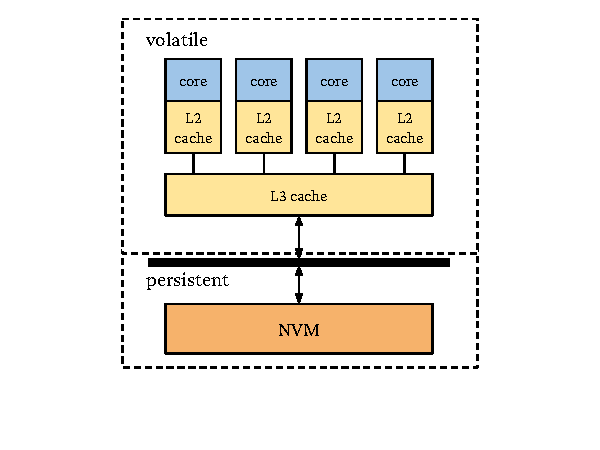
\includegraphics[width=\linewidth]{fig/vpdomains.pdf}
    \caption{Volatile and persistent domains on Intel CPUs. Once the memory controller has acknowledged the write, the system guarantees persistence of the write.}
    \label{fig:vpdomains}
\end{SCfigure}
\subsection{Bit Flipping}

\section{Distribution}

\unedit{
    Two fundamental changes arise as we distribute our data-centric system model---changes that present unavoidable challenges
    as well as new opportunities.  Given a multiplicity of loosely-coupled computers with independent storage and computing capabilities,
    we now need to consider both how data is \emph{shared} among computers, and how to schedule the \emph{rendezvous} between data
    and programs necessary to effect computation.

    It turns out that the key feature of Twizzler---explicit, context-free data identity---allows us to
    completely rethink system support for sharing and rendezvous because data and node identity are
    decoupled.
    It becomes easier to distribute applications, as they need not worry
    about coordinating a ``view'' of the object space across systems, nor do they need to worry about
    data movement when constructing data and relationships. We can more easily embed program
    logic in network, leveraging ``smarter'' network hardware because it can
    operate on data (in a limited way) without help from end-point applications. Computation can be
    created (or defined) on one machine and run transparently on another---a boon for edge-type
    systems---or can be paused and resumed elsewhere
    without synchronizing shared identity context, or even cooperatively partially executed
    by multiple machines.
}

\subsection{The Good Stuff}


\unedit{
    \subsubsection{Progressive and Immutable}

    %When objects do not change, or change in predictable ways, explicit identity enables powerful optimizations.
    %In this section, we expand on what it means for objects to change predictably.  We then provide examples of....

    %\subsection{Progressive and Immutable Objects}

    Of particular interest for optimizations are the class of \emph{progressive} objects.
    We call an object $O$ progressive if,
    given any two derived versions $O_1$ and $O_2$ of $O$, there is a unique object $O_m$ that incorporates all of the changes in $O_1$ and $O_2$.
    Immutable objects are trivially progressive, since they do not change.
    In the distributed systems literature, Conflict-free Replicated Datatypes
    (CRDTs)~\cite{shapiro2011comprehensive}
    are an important class of progressive objects.

    A system with explicit, context-free identity can unlock the power of progressive objects.
    These objects may always be replicated, and aggressively pushed towards
    sites where they are likely to be used.
    Anywhere along the way, divergent copies of progressive objects may be eagerly and automatically
    merged---even when the end-point applications that use the objects are nowhere to be found.

    % TODO: make sure this is talked about earlier
    Of course, the ``merge'' operation to compute $O_m$ may not be known to the OS; however, our
    ability to rendezvous both code and data throughout the system allows us to manifest the required
    applications where desired. Data objects themselves can identify what ``kind'' of object they are or
    what code objects are necessary to complete a merge.
    Thus if a particular node receives two divergent copies of a particular object, it can consult the
    object's metadata to determine what code to run to merge the two before forwarding the final object,
    $O_m$, all without consulting the end-point applications or performing some complex global
    coordination.

    %\todo[inline]{
    %Talk about how we can move around small pieces of "merge" code that can merge objects. Talk about
    %how objects can encode identifiers that describe what APIs they "respond" to.}

    \paragraph{Improving Prefetching}
    \label{sec:prefetch}

    Prefetching leverages spatial locality to improve future performance. A typical example is
    reading adjacent disk sectors under the assumption that their adjacency indicates that they
    will soon be needed. This example illustrates a common use of some proxy in place of actual data
    identity---this only works because file systems often try to lay out data in this way, and
    applications are optimized to take advantage of that layout. This, however, is \emph{extremely}
    fragile; the data may be unrelated, and the system cannot know this. Over a network, prefetching is
    often implemented in application specific ways, \eg, HTTP pushing additional resources that have
    not yet been requested. However, these relationships are, in general, undiscoverable by the system,
    limiting other applications to be beholden to each other in brittle ways
    and removing the benefits we could have with a more general automatic data movement
    model.

    When object relationships are explicit and can be interpreted to some extent by the
    system without help from applications, we can imagine an ``object graph'' that represents the
    relationships between objects. An example is shown in Figure~\ref{fig:ograph}, where
    an application has some ``root'' data object that refers to an index for a database, which in turn
    has references to data within some data object. Both the index and the data object (say they are
    CRDTs) provide the system with a reference to some merge code.

    Twizzler's FOT instantiates this object graph; it is understood by \emph{any} application
    and thus \emph{the system itself}.
    Of course, the system cannot have a
    perfect understanding of all the details of a data relationship---a particular external reference
    may be rarely used, or only used in a specific circumstance---but at least a translucent view of
    what objects may be accessed from a particular object can be useful to the system as a whole.

    \begin{SCfigure}[t]
        \centering
        \includegraphics[width=\linewidth]{genfig/obj_graph.pdf}
        \caption{Example object graph.}
        \label{fig:ograph}
    \end{SCfigure}

    An immediate consequence is that prefetching can be done based not on some proxy for identity,
    but instead on that identity itself. The system may not know for certain that object $A$ will
    reference object $B$, but it does know that it might, and will \emph{not} reference other objects.
    Because we have an end-to-end notion of identity, we can do this prefetching in the network itself,
    largely without application support.
    This dovetails nicely with progressive objects, as they enable aggressive pushing of objects around
    the system. Since object merging can be done \emph{anywhere}, it makes sense to prefetch objects
    more aggressively than in a system where this cannot be done.

}


\unedit{

    \subsection{Conventions Not Constraints}

    One might think we are suggesting all applications be written in a constrained data
    model, but this is not the case! While such a model has benefits as discussed above, it is
    important that our system design does not curtail applications' freedoms in how they design their
    data models. Many patterns in distributed systems require high-conflict objects (\eg mutexes), and
    while our system should provide benefits where possible it should not prevent these concepts from
    being represented.

    In particular, we support existing solutions and models. Traditional consistency and
    consensus algorithms that rely on machine identity to organize fault-tolerance zones still work (see
    Section~\ref{sec:name_machines}). Support for data with changing identity at run-time or data whose
    identity is not statically known can use late-binding, which our model explicitly makes
    allowances for (see Section~\ref{sec:latebinding}). Support for standard message-passing and RPC
    applications is encouraged by our model, as providing APIs to protect data access is a vital part of
    building complex systems; our end-to-end notion of identity facilitates this through the ability to
    refer to data without additional coordination. Objects with arbitrarily changing contents can be
    implemented through these methods, allowing applications like lock servers or complex databases to
    operate as usual.

    %While we get a significant benefit in a somewhat more constrained data model as discussed above, we realize that
    %not all systems and data fit that model. Thus it is important that we design our system in such a
    %way that we do not limit the generality and flexibility of applications that want to perform
    %arbitrary updates to data.

    %Of course there are challenges beyond those presented here; consistency and consensus, to name two examples,
    %are well studied and are we make no attempt to suggest that they should be ignored or replaced.
    %Indeed, our model makes room for allowing more complex applications to use these tools whenever
    %necessary.

    \subsubsection{Late-binding of Names}
    \label{sec:latebinding}

    A disadvantage of context-free references is the lack of late-binding of names,
    since late-binding occurs at the time that a reference is followed. This feature
    is vital, as it enables the construction of references to data that changes
    over-time (\eg shared libraries). While support for late-binding
    introduces \emph{some} context back into references, it does so in a controlled way. In Twizzler,
    instead of storing a GUID in an FOT entry, we can store a string and a reference
    to a name resolution function.
    This means
    that while a particular reference uses late-binding, the system can still compute the binding itself
    if necessary.

    Data relationships often do not require this.
    A common pattern is to construct some object graph (like
    Figure~\ref{fig:ograph}) and then name a single object as an ``entry point''.
    Names and late-binding in Twizzler are an overlay to data's actual
    identity, resulting in a ``two-level'' naming system that can use human-readable names to facilitate
    discovery for a more authoritative name (the GUID).
    %If a relationship between two object is ``tight'', then it would make sense to encode this
    %without late-binding. However, if a 


    %\todo[inline]{
    %Global name service ... }


    \subsubsection{Explicitly Naming Machines}
    \label{sec:name_machines}

    In our model, we usually refer to data without mixing machine identity into references,
    largely removing the need to identify machines themselves.
    However, at least for locality reasons,
    an application should be \emph{able} to identify and access a resource on a
    specific machine as part of its API---a particular
    %either run computation there or access data located on a \emph{specific} machine---a particular
    machine may control some physical device or resource or be an interface to some other system. This
    has been explored before~\cite{ousterhout:computer88,grapevine}; we explicitly allow for this
    throughout our system.

    Our model does not \emph{prevent} applications from adding notions of locality and
    machine identity to its API; instead, our goal is to move away from this as the \emph{default}
    construction.
    Twizzler has the ability to create ``control'' objects whose identities can be used
    where machine IDs or process IDs would normally be. This allows applications to talk about ephemeral
    actors with the same ``language'' as that of permanent data, which combines well with the
    late-binding mechanism discussed above. For example, applications could create references to ``the
    current coordinator node'' whose identity changes over-time.

    \subsubsection{Sharing in Heterogeneous Environments}

    Extending data structures through a heterogeneous environment is itself a challenge, as different
    machines interpret data in different ways. This is actually not a problem unique to distributed
    environments, however, as we see this cropping up in single-node systems as well. Of course, the
    ``explicit encoding of references as pointers'' model does \emph{not} require that all data be
    expressed as C structs. In fact, it is \emph{rarely} the case that complex distributed applications
    need or should have such a low-level view of data. Instead, higher-level languages that can already
    encode data in formats that allow for heterogeneous interpretation can also leverage explicit
    references as we have defined in our model.
}


\unedit{
    \subsubsection{more shit}
    \paragraph*{Decoupling Through Coupling.}
    %
    There is an irony in our vision for decoupling applications in a more
    flexible manner than RPC: this vision requires a \emph{stronger}
    coupling between the OS and the network.
    Pushing data identity into the OS and the network as a first-class
    abstraction has a number of benefits, but it does imply more rigidity
    in the lower-level infrastructure. We argue that this is okay, and even desirable. Our
    goal is to provide \emph{applications} with flexibility, scalability,
    and generality. By moving some application-level semantics
    like data references and identity into the lower-level system, we
    can implement in one place patterns like caching, prefetching, and
    query planning that often get reimplemented at many layers
    %(including
    %the application)
    \emph{because} these layers lack a common language to
    talk about data.
    %Our plan is to explore the trade-offs between lower level rigidity and application
    %flexibility.


    \paragraph*{Uniformity Between Code and Data.}
    %
    Recently, Wang et al.~\cite{wang:hotos21} proposed an extension to RPC
    that passes first class immutable references as well
    as values in procedure calls and returns.  The goal is to preserve the
    functional semantics of RPC while permitting the underlying system to
    avoid unnecessary copies and to perform memory management.  Their
    design is a step in the right direction, addressing some of the
    weaknesses of RPC, by making it possible for the system
    to transparently move data.  But, it only takes us halfway: RPC remains
    compute-centric and programmers must indicate
    \emph{where} code should execute.  For example, the optimization
    described in Section~\ref{sec:example} in which Dave (the powerful
    edge device) performs inference locally could not be realized via
    \emph{any} RPC mechanism.  In our system, code (like data) is global
    and referenceable from anywhere---there would be no reason to provide a
    separate mechanism for specifying function invocations. Instead, we
    place all data \emph{and} code in a single space, allowing code
    and data to reference each other. This dramatically improves
    expressivity, decoupling, and reuse, as we can now rely on the system
    to move not only data but also code to where it needs to be on demand
    without manual intervention and setup. In our model, the programmer
    primarily \emph{orchestrates a rendezvous between code and data}.


}
\subsection{The Hard Stuff}

\unedit{
    Running computations on a collection of loosely-coupled machines that fail independently raises the specter of
    \emph{partial failure}.  Machines may fail by crashing or becoming unreachable, conditions which
    can be difficult to detect. Care must be taken such that applications produce correct and complete
    results when partial failure is possible.  There have been decades of scholarship on
    fault tolerance~\cite{gray-dbos,3pc,bully,whydo,primary-site, primary-copy, thomas-quorum,paxos,zab}
    and we prefer to keep our design compatible with existing or emerging mechanisms rather than providing a single solution.
    We believe that the features of Twizzler---in particular, invariant, context-free data references---will simplify the implementations
    of existing fault-tolerance and durability mechanisms because they remove the need to update data
    when locations change and allows machines to participate in these algorithms with less
    application-specific global coordination.

    Many fault tolerance mechanisms employ \emph{replication} to guard against data loss that may occur
    due to component failure.
    Unfortunately, replicating data gives rise to \emph{consistency} concerns: ensuring that replicas agree on their state,
    or at least ensuring that they can eventually converge to a common state.  Like fault-tolerance, consistency of replicated data
    is a nuanced area.  We believe it would be a mistake to select a one-size-fits-all solution.  Instead our aim is to support
    %(and in
    %some cases facilitate)
    state-of-the-art and emerging solutions.
}

\unedit{
    \paragraph*{Limitations and Challenges.}
    %
    Many challenges lie ahead. Perhaps foremost among them is the tension between partial failure
    (inevitable in any distributed system), fault tolerance, and mechanisms that attempt to hide the
    movement of computation and data~\cite{waldo}.  Masking failures via replication gives rise to
    concerns about consistency; mechanisms that ensure consistency in the presence of possible conflicts
    are costly in general.  We plan to address these challenges along two separate axes. At the level of
    the system co-design, we will experiment with offloading some synchronization and
    arbitration~\cite{jin18,jepsen18} concerns to the programmable network (which now
    functions somewhat as a memory bus), letting us explore the consistency and coherence space
    together.  At the level of programming model, we will explore how a whole-system view of object
    identity and references can interface with languages to support patterns for weakly
    consistent replication, such as auto-merging progressive objects like
    CRDTs~\cite{shapiro2011comprehensive} during data movement.
}
\section{Addressing}

\subsection{Hardware As Active Substrate}

\subsection{Heterogeneous Computing}

